\documentclass[12pt]{article}
\usepackage[margin=2cm]{geometry}
\usepackage{amsmath}
\usepackage{graphicx}
\usepackage{slashed}

\begin{document}

\noindent
The following muon data is from Particle Data Group.%\footnote{\tt https://pdg.lbl.gov/2020/listings/rpp2020-list-muon.pdf}

\begin{center}
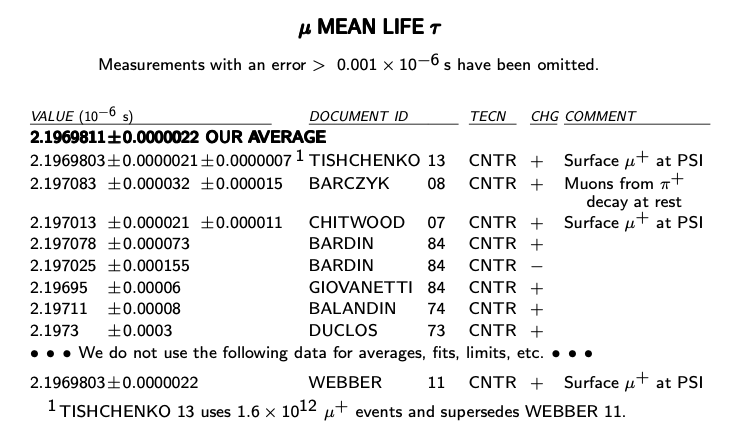
\includegraphics[scale=0.5]{muon-mean-life.png}
\end{center}

\noindent
From ``V minus A'' theory we have the following formula for muon lifetime $\tau$.
\begin{equation*}
\tau=\frac{96\pi^2h}{G_F^2\left(m_\mu c^2\right)^5}
\end{equation*}

\noindent
Symbol $G_F$ is Fermi coupling constant, $m_\mu$ is muon mass.

\bigskip
\noindent
From NIST we have
\begin{align*}
G_F&=1.1663787\times10^{-5}\;\text{GeV}^{-2}
\\
m_\mu&=1.883531627\times10^{-28}\;\text{kilogram}
\\
h&=6.62607015\times10^{-34}\;\text{joule}\;\text{second}\;\text{(exact)}
\\
c&=299792458\;\text{meter}\;\text{second}^{-1}\;\text{(exact)}
\\
1\,\text{eV}&=1.602176634\times10^{-19}\;\text{joule}\;\text{(exact)}
\end{align*}

\noindent
Hence
\begin{equation*}
\tau=\frac{96\pi^2h}{G_F^2\left(m_\mu c^2\right)^5}
=2.18735\times10^{-6}\,\text{second}
\end{equation*}

\noindent
The result is a bit smaller than the PDG value.
\begin{equation*}
\frac{\text{theoretical value}}{\text{measured value}}
=\frac{2.18735\times10^{-6}\,\text{second}}{2.19698\times10^{-6}\;\text{second}}=0.9956
\end{equation*}

\noindent
As the following diagram shows, a muon decays into a muon neutrino, an electron anti-neutrino,
and an electron.
\begin{center}
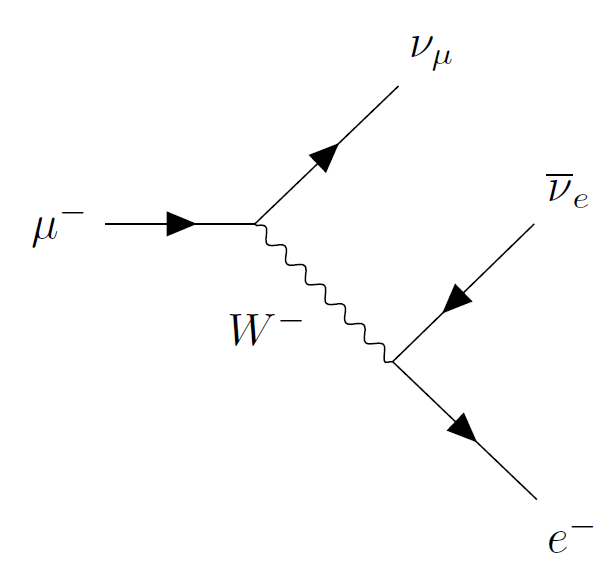
\includegraphics[scale=0.25]{muon-decay-diagram.png}
\end{center}

\begin{center}
\begin{tabular}{lllll}
Particle & Symbol & Momentum & Spinor (up) & Spinor (down)
\\[2ex]
Muon & $\mu^-$ & $p_1$ & $u_{11}$ & $u_{12}$
\\
Muon neutrino & $\nu_\mu$ & $p_2$ & $u_{21}$ & $u_{22}$
\\
Electron anti-neutrino & $\bar{\nu}_e$ & $p_3$ & $v_{31}$ & $v_{32}$
\\
Electron & $e^-$ & $p_4$ & $u_{41}$ & $u_{42}$
\end{tabular}
\end{center}

\noindent
We will use the following momentum vectors.
\begin{equation*}
p_1=
\underset{\substack{\\[1ex] \mu^-}}
{\begin{pmatrix}E_1\\p_{1x}\\p_{1y}\\p_{1z}\end{pmatrix}}
\qquad
p_2=
\underset{\substack{\\[1ex] \nu_\mu}}
{\begin{pmatrix}E_2\\p_{2x}\\p_{2y}\\p_{2z}\end{pmatrix}}
\qquad
p_3=
\underset{\substack{\\[1ex] \bar{\nu}_e}}
{\begin{pmatrix}E_3\\p_{3x}\\p_{3y}\\p_{3z}\end{pmatrix}}
\qquad
p_4=
\underset{\substack{\\[1ex] e^-}}
{\begin{pmatrix}E_4\\p_{4x}\\p_{4y}\\p_{4z}\end{pmatrix}}
\end{equation*}

\noindent
And we will use the following unnormalized Dirac spinors.
\begin{align*}
u_{11}&=
\underset{\substack{\\[1ex]\text{$\mu^-$ up}}}
{\begin{pmatrix}E_1+m_\mu\\0\\p_{1z}\\p_{1x}+ip_{1y}\end{pmatrix}}
&
u_{21}&=
\underset{\substack{\\[1ex]\text{$\nu_\mu$ up}}}
{\begin{pmatrix}E_2+m_2\\0\\p_{2z}\\p_{2x}+ip_{2y}\end{pmatrix}}
&
v_{31}&=
\underset{\substack{\\[1ex]\text{$\bar{\nu}_e$ up}}}
{\begin{pmatrix}p_{3z}\\p_{3x}+ip_{3y}\\E_3+m_3\\0\end{pmatrix}}
&
u_{41}&=
\underset{\substack{\\[1ex]\text{$e^-$ up}}}
{\begin{pmatrix}E_4+m_4\\0\\p_{4z}\\p_{4x}+ip_{4y}\end{pmatrix}}
\\[2ex]
u_{12}&=
\underset{\substack{\\[1ex]\text{$\mu^-$ down}}}
{\begin{pmatrix}0\\E_1+m_\mu\\p_{1x}-ip_{1y}\\-p_{1z}\end{pmatrix}}
&
u_{22}&=
\underset{\substack{\\[1ex]\text{$\nu_\mu$ down}}}
{\begin{pmatrix}0\\E_2+m_2\\p_{2x}-ip_{2y}\\-p_{2z}\end{pmatrix}}
&
v_{32}&=
\underset{\substack{\\[1ex]\text{$\bar{\nu}_e$ down}}}
{\begin{pmatrix}p_{3x}-ip_{3y}\\-p_{3z}\\0\\E_3+m_3\end{pmatrix}}
&
u_{42}&=
\underset{\substack{\\[1ex]\text{$e^-$ down}}}
{\begin{pmatrix}0\\E_4+m_4\\p_{4x}-ip_{4y}\\-p_{4z}\end{pmatrix}}
\end{align*}

\noindent
Symbol $E_n$ is total energy of particle $n$.
\begin{align*}
E_1&=\sqrt{(p_{1x})^2+(p_{1y})^2+(p_{1z})^2+m_\mu^2}
\\
E_2&=\sqrt{(p_{2x})^2+(p_{2y})^2+(p_{2z})^2+m_2^2}
\\
E_3&=\sqrt{(p_{3x})^2+(p_{3y})^2+(p_{3z})^2+m_3^2}
\\
E_4&=\sqrt{(p_{4x})^2+(p_{4y})^2+(p_{4z})^2+m_4^2}
\end{align*}

\noindent
From the Feynman diagram above we have the following amplitude $\mathcal{M}_{abcd}$
where each letter in $abcd$ can be either 1 (spin up) or 2 (spin down).
\begin{equation*}
\mathcal{M}_{abcd}=\frac{G_F}{\sqrt{2}\sqrt{N}}
\big(
\underset{\substack{\\[1ex]e^-}}{\bar{u}_{4d}}
\;
\underset{\substack{\\[1ex] }}{\gamma^\mu(1-\gamma^5)}
\;
\underset{\substack{\\[1ex]\bar{\nu}_e}}{v_{3c}}
\big)
\big(
\underset{\substack{\\[1ex]\nu_\mu}}{\bar{u}_{2b}}
\;
\underset{\substack{\\[1ex] }}{\gamma_\mu(1-\gamma^5)}
\;
\underset{\substack{\\[1ex]\mu^-}}{u_{1a}}
\big)
\end{equation*}

\noindent
Symbol $N$ is the following spinor normalization constant.
\begin{equation*}
N=(E_1+m_\mu)(E_2+m_2)(E_3+m_3)(E_4+m_4)
\end{equation*}

\noindent
Recall that the magnitude squared of an amplitude is a probability density and also an observable.
\begin{equation*}
|\mathcal{M}_{abcd}|^2=\mathcal{M}_{abcd}^*\mathcal{M}_{abcd}
\end{equation*}

\noindent
In a typical muon decay experiment the spins are not observed.
Consequently, the experimental result is an average of spin states.
The average is computed by summing over all spin states and dividing by the number of initial spin states.
The muon has two spin states hence the divisor is two.
\begin{equation*}
\langle|\mathcal{M}|^2\rangle=
\frac{1}{2}
\sum_{a=1}^2\sum_{b=1}^2\sum_{c=1}^2\sum_{d=1}^2
|\mathcal{M}_{abcd}|^2
\end{equation*}

\noindent
The result is a simple formula.
\begin{equation*}
\langle|\mathcal{M}|^2\rangle=64G_F^2(p_1\cdot p_3)(p_2\cdot p_4)
\tag{1}
\end{equation*}

\noindent
In component notation we have
\begin{equation*}
\langle|\mathcal{M}|^2\rangle=64G_F^2
(p_1^\mu \, g_{\mu\nu} \, p_3^\nu)
(p_2^\rho \, g_{\rho\sigma} \, p_4^\sigma)
\end{equation*}
where
\begin{equation*}
g_{\mu\nu}=g_{\rho\sigma}=\begin{pmatrix}
1 & 0 & 0 & 0\\
0 & -1 & 0 & 0\\
0 & 0 & -1 & 0\\
0 & 0 & 0 & -1
\end{pmatrix}
\end{equation*}

\noindent
Muon decay rate $\Gamma$ is essentially an expectation value (weighted average)
for all possible values of particle momentum.
In the muon rest frame we have $p_1=(m_\mu,0,0,0)$ and by Fermi's golden rule
\begin{equation*}
\Gamma=\frac{1}{512\pi^5m_\mu}
\int\limits_{-\infty}^\infty \cdots \int\limits_{-\infty}^\infty
\langle|\mathcal{M}|^2\rangle
\,\delta(p_1-p_2-p_3-p_4)
\,\frac{d^3p_2}{E_2}\,\frac{d^3p_3}{E_3}\,\frac{d^3p_4}{E_4}
\end{equation*}

\noindent
Altogether there are nine integrals, three for each of $p_2$, $p_3$, and $p_4$.
The delta function restricts the integration space to values that conserve energy and momentum.

\bigskip
\noindent
It can be shown that
\begin{equation*}
\Gamma=\frac{G_F^2 m_\mu^5}{192\pi^3}
\end{equation*}

\noindent
Muon lifetime $\tau$ is the inverse of decay rate.
\begin{equation*}
\tau=\frac{1}{\Gamma}=\frac{192\pi^3}{G_F^2 m_\mu^5}
\end{equation*}

\noindent
Converting from natural units to physical values for $h$ and $c$ yields
\begin{equation*}
\tau
=\frac{192\pi^3\hbar}{G_F^2\left(m_\mu c^2\right)^5}
=\frac{96\pi^2h}{G_F^2\left(m_\mu c^2\right)^5}
\end{equation*}

\noindent
Probability density $\langle|\mathcal{M}|^2\rangle$ can also be computed
using the following Casimir trick.
\begin{equation*}
\langle|\mathcal{M}|^2\rangle
=\frac{G_F^2}{4}
\mathop{\text{Tr}}
\left(\slashed{p}_4\gamma^\mu(1-\gamma^5)\slashed{p}_3\gamma^\nu(1-\gamma^5)\right)
\mathop{\text{Tr}}
\left(\slashed{p}_2\gamma_\mu(1-\gamma^5)\slashed{p}_1\gamma_\nu(1-\gamma^5)\right)
\end{equation*}

\noindent
The slashed symbols are $4\times4$ matrices computed as
\begin{equation*}
\slashed{p}=p\cdot\gamma
=p^0\gamma^0-p^1\gamma^1-p^2\gamma^2-p^3\gamma^3
\end{equation*}

\noindent
For example,
\begin{equation*}
\slashed{p}_1=\begin{pmatrix}
E_1 & 0 & -p_{1z} & -p_{1x} + ip_{1y}
\\[1ex]
0 & E_1 & -p_{1x} - ip_{1y} & p_{1z}
\\[1ex]
p_{1z} & p_{1x} - i p_{1y} & -E_1 & 0
\\[1ex]
p_{1x} + ip_{1y} & -p_{1z} & 0 & -E_1
\end{pmatrix}
\end{equation*}

\end{document}
